\section{Classical Wave Equation}

\begin{frame}{Title}
    Our first goal is to approximate the solution of

    \begin{equation*}
        \fcolorbox{BrickRed}{white}{$\displaystyle\frac{\partial^2u}{\partial t^2}-c^2\frac{\partial^2u}{\partial x^2}=0$} \ \longleftarrow \ \text{\textbf{\textcolor{BrickRed}{d'Alembert equation}}}
    \end{equation*}

    \vfill

    \begin{figure}[H]
        \centering
        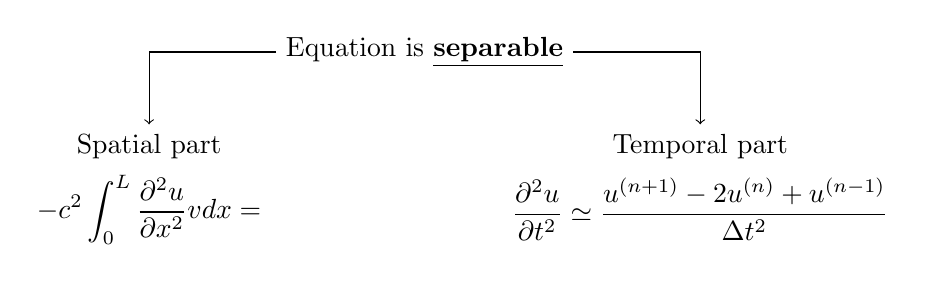
\begin{tikzpicture}
            \node at (0,3) (A) {Equation is \underline{\textbf{separable}}};
            \node at (-3.5,1.8) (B) {Spatial part};
            \node at (3.5,1.8) (C) {Temporal part};
            \node at (-3.5,1) (D) {$\displaystyle-c^2\int_0^L\frac{\partial^2u}{\partial x^2}vdx=$};
            \node at (3.5,1) (E) {$\displaystyle\frac{\partial^2u}{\partial t^2}\simeq\frac{u^{(n+1)}-2u^{(n)}+u^{(n-1)}}{\Delta t^2}$};

            \draw[->] (A) -- (-3.5,3) -- (B);
            \draw[->] (A) -- (3.5,3) -- (C);
        \end{tikzpicture}
    \end{figure}
\end{frame}